\documentclass[10pt,twocolumn,letterpaper]{article}
\usepackage[top=0.75in,bottom=0.9in,left=0.625in,right=0.625in,columnsep=0.25in]{geometry}
\usepackage[T1]{fontenc}
\usepackage{mathptmx}
\usepackage[scaled=.92]{helvet}
\usepackage{amsmath,amssymb}
\usepackage{booktabs,graphicx,array}
\usepackage{microtype}
\usepackage{tikz}
\usetikzlibrary{arrows.meta,positioning,fit,backgrounds,calc}

\usepackage{caption}\usepackage{makecell}
\usepackage{titlesec}
\usepackage[bookmarks=false,colorlinks=false,pdfborder={0 0 0}]{hyperref}
\usepackage{cite}
\usepackage{balance}

% ---- IEEE-conference-style look ----
\setlength{\parindent}{1.0em}
\setlength{\parskip}{0pt}
\renewcommand{\thesection}{\Roman{section}}
\renewcommand{\thesubsection}{\Alph{subsection}}
\titleformat{\section}{\centering\normalfont\small\scshape}{\thesection.}{0.6em}{}
\titleformat{\subsection}{\normalfont\itshape}{\thesubsection.}{0.5em}{}
\titlespacing*{\section}{0pt}{7pt}{3pt}
\titlespacing*{\subsection}{0pt}{4pt}{1.5pt}
\renewcommand{\figurename}{Fig.}
\renewcommand{\tablename}{TABLE}
\renewcommand{\thetable}{\Roman{table}}
\captionsetup[figure]{labelfont=rm,textfont=rm,labelsep=period,font=footnotesize,justification=justified,singlelinecheck=true}
\captionsetup[table]{labelfont=sc,textfont=sc,labelsep=newline,font=footnotesize,justification=centering,skip=3pt}
\setlength{\abovedisplayskip}{3pt}\setlength{\belowdisplayskip}{3pt}
\setlength{\abovedisplayshortskip}{2pt}\setlength{\belowdisplayshortskip}{2pt}
\setlength{\textfloatsep}{8pt plus 2pt minus 2pt}
\setlength{\floatsep}{6pt plus 2pt minus 2pt}
\setlength{\intextsep}{6pt plus 2pt minus 2pt}
\pagestyle{empty}
\sloppy

\newcommand{\ie}{\textit{i.e.}}
\newcommand{\eg}{\textit{e.g.}}

\begin{document}

\twocolumn[
\begin{@twocolumnfalse}
\centering
{\fontsize{22}{24}\selectfont Architecture of Kimi K2: An Ultra-Sparse Mixture-of-Experts Language Model for Agentic Intelligence\par}
\vspace{6pt}

\vspace{6pt}
\begin{minipage}{6.9in}
\small\bfseries
\noindent\textit{Abstract}---Kimi K2 is an open-weight Mixture-of-Experts (MoE) large language model from Moonshot AI with 1.04 trillion total and 32.6 billion activated parameters, built for agentic intelligence. This paper analyzes its architecture using the official technical report and the prior work it builds on. We examine (i) the ultra-sparse MoE layer (384 routed experts, 8 activated per token, plus one shared expert), (ii) Multi-head Latent Attention (MLA) with the head count halved to 64, (iii) the MuonClip optimizer, whose QK-Clip rule bounds attention logits and allowed 15.5T-token pre-training without a single loss spike, and (iv) the agentic data-synthesis and joint reinforcement-learning pipeline used in post-training. We quantify the parameter budget, per-token compute and long-context KV-cache footprint, compare K2 with DeepSeek-V3 in structure and benchmark results, and identify the innovations that distinguish it from other MoE language models.

\vspace{4pt}
\noindent\textit{Index Terms}---Kimi K2, mixture of experts, multi-head latent attention, Muon optimizer, QK-Clip, large language models, agentic intelligence.
\end{minipage}
\vspace{6pt}
\end{@twocolumnfalse}
]

\section{Introduction and Model Overview}
Kimi K2 \cite{kimik2} is a large language model developed by Moonshot AI (the Kimi Team) and released in July 2025 as open-weight base (Kimi-K2-Base) and post-trained (Kimi-K2-Instruct) checkpoints. It succeeds the Kimi k1.5 reinforcement-learning line \cite{k15} and targets \emph{agentic intelligence}: the ability to plan, use tools, and act over many steps, with particular strength in software engineering and tool-use workloads. Architecturally, K2 is a decoder-only Transformer \cite{vaswani} that follows the DeepSeek-V3 template \cite{dsv3}---MLA attention and a fine-grained MoE feed-forward network---but re-tunes it through scaling-law analysis: more experts, half as many attention heads, and fewer dense layers. The report treats \emph{token efficiency} (learning signal per training token) as the central design axis, which motivates the Muon optimizer, synthetic data rephrasing, and reinforcement learning. Section~II details the architecture, Section~III the training methodology, Section~IV inference and performance, and Section~V the innovations relative to DeepSeek-V3 and other MoE models.

\begin{figure*}[!t]
\centering
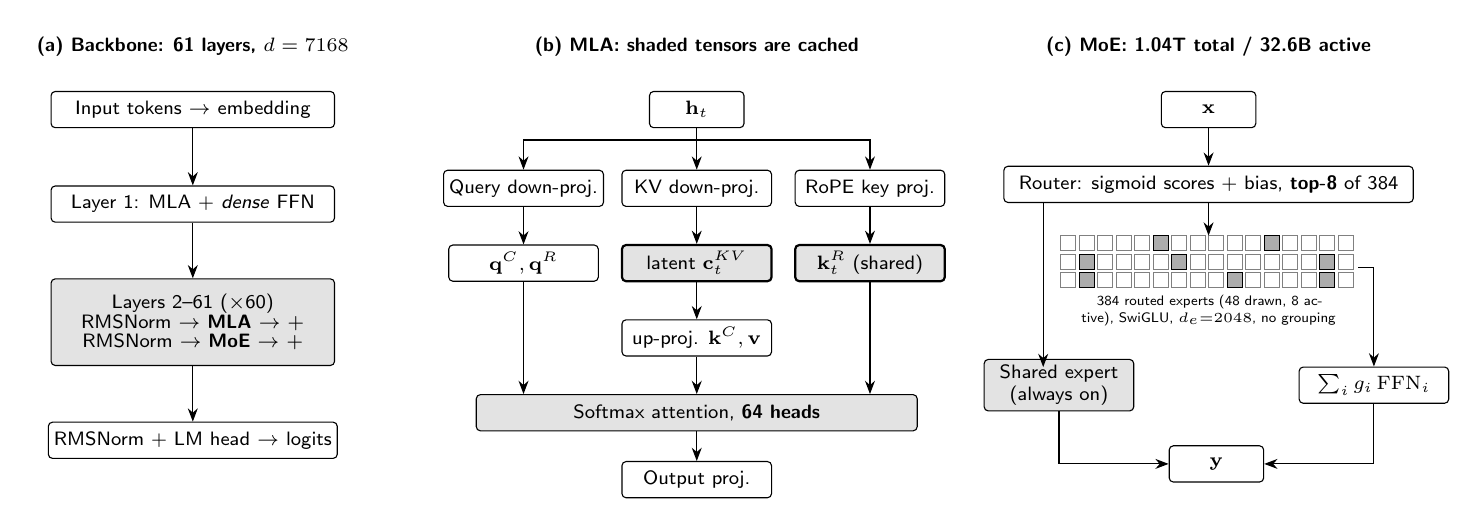
\begin{tikzpicture}[
  font=\sffamily\scriptsize, >=Stealth,
  box/.style={draw, rounded corners=1.5pt, minimum height=4.6mm, align=center, inner sep=2pt, line width=0.4pt, fill=white},
  hot/.style={box, fill=gray!22},
  cache/.style={box, fill=gray!22, line width=0.8pt},
  ptitle/.style={font=\sffamily\scriptsize\bfseries},
  arr/.style={->, line width=0.4pt}
]
% ---------- (a) backbone ----------
\node[ptitle] at (2.0,0.8) {(a) Backbone: 61 layers, $d=7168$};
\node[box, minimum width=3.6cm] (a0) at (2.0,0) {Input tokens $\rightarrow$ embedding};
\node[box, minimum width=3.6cm] (a1) at (2.0,-1.2) {Layer 1: MLA + \emph{dense} FFN};
\node[hot, minimum width=3.6cm, minimum height=11mm] (a2) at (2.0,-2.7) {Layers 2--61 ($\times$60)\\[-1pt]RMSNorm $\rightarrow$ \textbf{MLA} $\rightarrow$ $+$\\[-1pt]RMSNorm $\rightarrow$ \textbf{MoE} $\rightarrow$ $+$};
\node[box, minimum width=3.6cm] (a3) at (2.0,-4.2) {RMSNorm + LM head $\rightarrow$ logits};
\draw[arr] (a0)--(a1); \draw[arr] (a1)--(a2); \draw[arr] (a2)--(a3);

% ---------- (b) MLA ----------
\node[ptitle] at (8.4,0.8) {(b) MLA: shaded tensors are cached};
\node[box, minimum width=1.2cm] (h) at (8.4,0) {$\mathbf{h}_t$};
\node[box, minimum width=1.9cm] (qp) at (6.2,-1.0) {Query down-proj.};
\node[box, minimum width=1.9cm] (kvp) at (8.4,-1.0) {KV down-proj.};
\node[box, minimum width=1.9cm] (krp) at (10.6,-1.0) {RoPE key proj.};
\node[box, minimum width=1.9cm] (cq) at (6.2,-1.95) {$\mathbf{q}^C,\mathbf{q}^R$};
\node[cache, minimum width=1.9cm] (ckv) at (8.4,-1.95) {latent $\mathbf{c}^{KV}_t$};
\node[cache, minimum width=1.9cm] (kr) at (10.6,-1.95) {$\mathbf{k}^R_t$ (shared)};
\node[box, minimum width=1.9cm] (up) at (8.4,-2.9) {up-proj. $\mathbf{k}^C,\mathbf{v}$};
\node[hot, minimum width=5.6cm] (att) at (8.4,-3.85) {Softmax attention, \textbf{64 heads}};
\node[box, minimum width=1.9cm] (op) at (8.4,-4.7) {Output proj.};
\draw[arr] (h.south)--++(0,-0.15)-|(qp.north);
\draw[arr] (h.south)--(kvp.north);
\draw[arr] (h.south)--++(0,-0.15)-|(krp.north);
\draw[arr] (qp)--(cq); \draw[arr] (kvp)--(ckv); \draw[arr] (krp)--(kr);
\draw[arr] (ckv)--(up);
\draw[arr] (cq.south)--(cq.south |- att.north);
\draw[arr] (up.south)--(up.south |- att.north);
\draw[arr] (kr.south)--(kr.south |- att.north);
\draw[arr] (att)--(op);

% ---------- (c) MoE ----------
\node[ptitle] at (14.9,0.8) {(c) MoE: 1.04T total / 32.6B active};
\node[box, minimum width=1.2cm] (x) at (14.9,0) {$\mathbf{x}$};
\node[box, minimum width=5.2cm] (rt) at (14.9,-0.95) {Router: sigmoid scores + bias, \textbf{top-8} of 384};
\begin{scope}[shift={(13.02,-1.6)}]
  \foreach \r in {0,1,2}{
    \foreach \c in {0,...,15}{
      \pgfmathtruncatemacro{\id}{\r*16+\c}
      \pgfmathtruncatemacro{\sel}{(\id==5 || \id==11 || \id==17 || \id==22 || \id==30 || \id==33 || \id==41 || \id==46)?1:0}
      \ifnum\sel=1
        \fill[gray!65, draw=black, line width=0.3pt] (\c*0.235,-\r*0.235) rectangle ++(0.19,-0.19);
      \else
        \draw[line width=0.3pt, gray] (\c*0.235,-\r*0.235) rectangle ++(0.19,-0.19);
      \fi
    }
  }
\end{scope}
\node[align=center, text width=3.7cm, font=\sffamily\tiny] at (14.9,-2.55) {384 routed experts (48 drawn, 8 active), SwiGLU, $d_e{=}2048$, no grouping};
\node[hot, minimum width=1.9cm] (sh) at (13.0,-3.5) {Shared expert\\(always on)};
\node[box, minimum width=1.9cm] (sm) at (17.0,-3.5) {$\sum_i g_i\,\mathrm{FFN}_i$};
\node[box, minimum width=1.2cm] (y) at (15.0,-4.5) {$\mathbf{y}$};
\draw[arr] (x)--(rt);
\draw[arr] (rt.south)--(14.9,-1.6);
\draw[arr] (12.8,-1.18)--(12.8,-3.27);
\draw[arr] (16.8,-2.0) -| (sm.north);
\draw[arr] (sh.south) |- (y.west);
\draw[arr] (sm.south) |- (y.east);
\end{tikzpicture}

\caption{Kimi K2 architecture. (a) Backbone with one dense and 60 MoE layers. (b) MLA caches only a compressed latent and a shared rotary key per token. (c) Each token is routed to 8 of 384 experts plus one shared expert.}
\label{fig:arch}
\end{figure*}

\section{Architecture}
\subsection{Specification and Parameter Budget}
K2 has 61 Transformer layers, hidden dimension 7168, and expert hidden dimension 2048; only the first layer uses a dense FFN \cite{kimik2}. Table~\ref{tab:arch} compares it with DeepSeek-V3. Total parameters grow 54\% to 1.04T while activated parameters fall 13\% to 32.6B, so only 3.1\% of weights participate in any forward pass. A SwiGLU expert has $3\,d\,d_e = 3\cdot7168\cdot2048\approx 44.0$M parameters, so the $60\times384$ routed experts hold $\approx$1.015T parameters (97.6\% of the model), while the nine experts a token uses per layer (8 routed + 1 shared) account for $\approx$23.8B of the 32.6B activated; the remaining $\approx$8.8B (by subtraction) lies in attention, the dense layer, and embeddings. These figures are our derivation from the published dimensions.

\begin{table}[!t]
\caption{Architecture of Kimi K2 vs.\ DeepSeek-V3 \cite{kimik2}}
\label{tab:arch}
\centering\footnotesize
\setlength{\tabcolsep}{4pt}
\begin{tabular}{lccc}
\toprule
 & DeepSeek-V3 & Kimi K2 & $\Delta$ \\
\midrule
Layers & 61 & 61 & = \\
Total / activated params & 671B / 37B & 1.04T / 32.6B & $\uparrow$54\% / $\downarrow$13\% \\
Routed experts (total) & 256 & 384 & $\uparrow$50\% \\
Experts active per token & 8 & 8 & = \\
Shared experts & 1 & 1 & = \\
Sparsity (total/active) & 32 & 48 & $\uparrow$50\% \\
Attention heads & 128 & 64 & $\downarrow$50\% \\
Dense layers & 3 & 1 & $\downarrow$67\% \\
Expert grouping & Yes & No & -- \\
\bottomrule
\end{tabular}
\end{table}

\subsection{Mixture of Experts and Routing}
Sparse expert layers \cite{shazeer,gshard} decouple capacity from per-token compute. For a token with hidden state $\mathbf{x}$ the MoE layer of K2 computes, following the DeepSeek-V3 formulation \cite{dsv3} on which its design is based,
\begin{equation}
\mathbf{y}=\mathrm{FFN}_{s}(\mathbf{x})+\sum_{i\in\mathcal{T}(\mathbf{x})} g_i(\mathbf{x})\,\mathrm{FFN}_i(\mathbf{x}),\quad
g_i=\frac{s_i}{\sum_{j\in\mathcal{T}}s_j},
\end{equation}
where $s_i=\sigma(\mathbf{u}_i^{\!\top}\mathbf{x})$ is the sigmoid affinity to expert $i$, $\mathcal{T}(\mathbf{x})=\mathrm{TopK}_{8}\{s_i+b_i\}$ selects eight of 384 routed experts, and $b_i$ is a load-balancing bias used only for selection in \cite{dsv3}. The technical report confirms top-8 selection, one always-active shared expert, and, unlike DeepSeek-V3, no expert grouping \cite{kimik2}; it does not restate the router internals, so they are taken from \cite{dsv3}. Sparsity is defined as
\begin{equation}
S=\frac{E_{\text{routed}}}{k}=\frac{384}{8}=48.
\end{equation}
A sparsity scaling law fitted under Muon shows that, at constant activated parameters, higher sparsity lowers training and validation loss; to reach validation loss 1.5, $S{=}48$ needs $1.69\times$, $1.39\times$ and $1.15\times$ fewer FLOPs than $S{=}8$, 16 and 32 \cite{kimik2}. $S{=}48$ was chosen as the balance between this gain and the extra infrastructure complexity.

\subsection{Attention and Long-Context Handling}
K2 uses Multi-head Latent Attention \cite{dsv2}, which compresses keys and values into a low-rank latent:
\begin{equation}
\mathbf{c}^{KV}_t=W^{DKV}\mathbf{h}_t,\;\;
\mathbf{k}^{C}_t=W^{UK}\mathbf{c}^{KV}_t,\;\;
\mathbf{v}_t=W^{UV}\mathbf{c}^{KV}_t,
\end{equation}
with a separate decoupled rotary key $\mathbf{k}^R_t$ shared across heads. Only $\mathbf{c}^{KV}_t$ and $\mathbf{k}^R_t$ are cached. Assuming DeepSeek-V3's latent sizes ($d_c{=}512$, $d_R{=}64$), the cache is $L(d_c{+}d_R)=61\cdot576$ values per token---about 70\,KB in BF16, or roughly 9.2\,GB for one 128K-token sequence, about $28\times$ smaller than caching full 64-head keys and values (derived).

The main departure from DeepSeek-V3 is the head count: 64 instead of 128 \cite{kimik2}. At 128K context, doubling heads (with 384 experts) raises inference FLOPs by 83\%, yet only improves validation loss by 0.5--1.2\% under iso-token training, so K2 keeps 64. Long context is obtained in training: pre-training uses 4K sequences, annealing adds 60B tokens at 32K, and YaRN \cite{yarn} extends the window to 128K.

\section{Training Methodology}
\subsection{MuonClip Optimizer}
K2 is trained with Muon \cite{muon,muonscale}, which orthogonalizes the momentum update by Newton--Schulz iteration and rescales it to match AdamW's update RMS:
\begin{equation}
\begin{split}M_t&=\mu M_{t-1}+G_t,\quad O_t=\mathrm{NS}(M_t)\sqrt{\max(n,m)}\,0.2,\\ W_t&=W_{t-1}-\eta(O_t+\lambda W_{t-1}).\end{split}
\end{equation}
Muon is more token-efficient than AdamW but made attention logits explode: in a 9B-active/53B-total run they exceeded 1000. QK-Norm \cite{qknorm} cannot be used with MLA because keys are not materialized at inference, and logit soft-capping acts too late. K2 therefore adds \emph{QK-Clip}, which rescales the query/key weights after each update whenever a head's maximum logit $S^h_{\max}$ exceeds a threshold $\tau$:
\begin{equation}
\gamma_h=\min\!\Big(1,\frac{\tau}{S^h_{\max}}\Big),\quad W^h_{q^C},W^h_{k^C}\!\leftarrow\!\sqrt{\gamma_h}\,(\cdot),\quad W^h_{q^R}\!\leftarrow\!\gamma_h\,W^h_{q^R},
\end{equation}
applied per head and leaving the shared rotary key untouched \cite{kimik2}. With $\tau{=}100$, 12.7\% of heads triggered clipping in the first 70K steps, after which all logits fell below the cap and QK-Clip became inactive. Muon plus QK-Clip is called MuonClip, and K2 completed 15.5T tokens with zero loss spikes.

\subsection{Data, Schedule and Infrastructure}
The 15.5T-token corpus spans web text, code, mathematics, and knowledge. To raise token utility, high-quality text is \emph{rephrased} with style-diverse prompts, chunk-wise autoregressive rewriting, and fidelity checks \cite{wrap,kimik2}; on SimpleQA, one rephrasing with 10 epochs raised accuracy from 23.76 to 27.39, and 10 rephrasings in one epoch to 28.94. The schedule is warmup--stable--decay \cite{wsd}: 10T tokens at constant $2\times10^{-4}$, 5.5T tokens of cosine decay to $2\times10^{-5}$, weight decay 0.1, and a 67M-token batch, followed by annealing to $7\times10^{-6}$ (400B tokens at 4K, 60B at 32K).

Training ran on NVIDIA H800 nodes (8 GPUs with NVLink/NVSwitch, 2\,TB RAM, 8$\times$400\,Gb/s RoCE) with 16-way pipeline parallelism with virtual stages, 16-way expert parallelism, and ZeRO-1 data parallelism \cite{zero,megatron}. Parameters (BF16) plus FP32 gradient buffers need $\approx$6\,TB across a 256-GPU model-parallel group ($\approx$30\,GB per GPU). K2 uses interleaved 1F1B rather than DualPipe, the smallest workable EP size, selective recomputation, FP8 storage of insensitive activations, and CPU offloading \cite{kimik2}.

\subsection{Post-Training and Reinforcement Learning}
Supervised fine-tuning also uses Muon. A large-scale agentic synthesis pipeline builds a repository of 3000+ real MCP tools and 20{,}000+ synthetic tools, generates agents and rubric-bearing tasks, simulates users and tool environments, and keeps only trajectories accepted by an LLM judge; real sandboxes (10{,}000+ concurrent instances) supply ground truth for coding. Reinforcement learning combines verifiable rewards (math, STEM, logic, instruction following, coding, faithfulness, safety) with a \emph{self-critique rubric reward} for subjective tasks, where the model ranks its own outputs pairwise. The policy objective of Kimi k1.5 \cite{k15} is used,
\begin{equation}
\mathcal{L}_{\mathrm{RL}}(\theta)=\mathbb{E}_{x}\Big[\tfrac1K\textstyle\sum_{i=1}^{K}\Big(r(x,y_i)-\bar r(x)-\tau\log\tfrac{\pi_\theta(y_i|x)}{\pi_{\mathrm{old}}(y_i|x)}\Big)^{2}\Big],
\end{equation}
with a per-task token budget penalty, an auxiliary PTX loss against forgetting, and temperature decay. A colocated train/inference design with a checkpoint engine updates all weights in under 30\,s \cite{kimik2}.

\section{Inference and Performance}
\subsection{Efficiency, Memory and Scalability}
Per-token matrix compute scales with activated, not total, parameters: roughly $2\times32.6$B $\approx$65\,GFLOPs, plus attention terms that grow with context (derived). Halving heads directly cuts the attention part; the 83\% FLOP increase quoted above is the cost K2 avoids at 128K. Memory is governed by total parameters: the weights alone need about 1.04\,TB at 8 bits per parameter (2.1\,TB in BF16), so serving is multi-node, with expert-parallel all-to-all communication, and sparse activation makes decoding bandwidth-bound rather than compute-bound. The MLA cache (about 9.2\,GB per 128K sequence, Section II-C) keeps batch size feasible at long context. The report does not publish serving throughput or latency figures, so none are claimed here.

\subsection{Benchmark Performance}
Table~\ref{tab:bench} lists developer-reported non-thinking results at release \cite{kimik2}. K2 leads open models on every row and exceeds Claude Opus~4 on LiveCodeBench, AIME~2025 and GPQA-Diamond, but trails it on SWE-bench Verified (65.8 vs.\ 72.5; 71.6 with multiple attempts) and MMLU. It also reached 66.1 on $\tau^2$-Bench and was ranked first among open models and fifth overall on LMSYS Arena (July 17, 2025). Kimi-K2-Base beats DeepSeek-V3-Base on MMLU (87.79 vs.\ 87.10) and EvalPlus (80.33 vs.\ 65.61). Noted limitations are excess tokens on hard reasoning or ambiguous tools and weaker one-shot project generation.

\begin{table}[!t]
\caption{Reported Non-Thinking Benchmark Results \cite{kimik2}}
\label{tab:bench}
\centering\footnotesize
\setlength{\tabcolsep}{2.6pt}
\begin{tabular}{lccccc}
\toprule
Benchmark & \makecell{Kimi\\K2} & \makecell{DS-V3\\0324} & \makecell{Qwen3\\235B} & \makecell{Claude\\Opus 4} & \makecell{GPT\\4.1} \\
\midrule
SWE-bench Verified (agentic) & \textbf{65.8} & 38.8 & 34.4 & 72.5 & 54.6 \\
SWE-bench Multilingual & \textbf{47.3} & 25.8 & 20.9 & --- & 31.5 \\
LiveCodeBench v6 & \textbf{53.7} & 46.9 & 37.0 & 47.4 & 44.7 \\
$\tau^2$-Bench Telecom & \textbf{65.8} & 32.5 & 22.1 & 57.0 & 38.6 \\
ACEBench (en) & 76.5 & 72.7 & 70.5 & 75.6 & \textbf{80.1} \\
AIME 2025 (Avg@64) & \textbf{49.5} & 46.7 & 24.7 & 33.9 & 37.0 \\
GPQA-Diamond & \textbf{75.1} & 68.4 & 62.9 & 74.9 & 66.3 \\
MMLU (EM) & 89.5 & 89.4 & 87.0 & \textbf{92.9} & 90.4 \\
\bottomrule
\end{tabular}
\end{table}

\section{Architectural Innovations}
\subsection{Distinguishing Features}
Relative to DeepSeek-V3 and other MoE models, K2's contributions are:
\emph{(1) Ultra-sparsity}: sparsity 48 yields a total-to-active ratio of about 32, versus 18 for DeepSeek-V3 (671B/37B), 24 for Llama~4 Maverick (400B/17B) and 11 for Qwen3-235B-A22B. 
\emph{(2) Inference-driven attention}: 64 heads trade a $\le$1.2\% loss gain for large long-context savings. 
\emph{(3) Simpler stack}: one dense layer instead of three, and no expert grouping. 
\emph{(4) MuonClip}: Muon-family training reported stable at trillion-parameter scale over 15.5T tokens, using a self-deactivating rule that avoids QK-Norm. 
\emph{(5) Token-efficiency data and agentic post-training}: rephrasing, large-scale tool-use synthesis, and RL with verifiable plus self-critique rewards.

\subsection{Interaction of Components}
The components are coupled. Higher sparsity raises all-to-all traffic, so K2 needs the smallest EP group; but fewer heads shorten attention time, leaving less computation to hide that traffic, which reinforces choosing EP${=}16$ with interleaved 1F1B. Muon's token efficiency raises logit-explosion risk; MLA rules out QK-Norm; hence QK-Clip acts directly on MLA's unshared query/key components. Finally, MLA's compact cache plus 64 heads keeps long agentic trajectories affordable, which the synthetic-data and RL stages then exploit.

\section{Conclusion}
Kimi K2 shows that a DeepSeek-V3-style MLA+MoE backbone can be pushed to 1.04T parameters at 32.6B active by combining ultra-sparse routing, a leaner attention configuration, and a stability-aware optimizer. Its main design lesson is that architecture, optimizer, and infrastructure must be co-designed. Reported results are developer-measured at release; independent replication and published serving benchmarks would strengthen the analysis.

\balance
\begingroup
\footnotesize
\begin{thebibliography}{99}\setlength{\itemsep}{0pt}\setlength{\parsep}{0pt}
\bibitem{kimik2} Kimi Team, ``Kimi K2: Open agentic intelligence,'' arXiv:2507.20534, 2025 (v2, Feb.\ 2026).
\bibitem{k15} Kimi Team, ``Kimi k1.5: Scaling reinforcement learning with LLMs,'' arXiv:2501.12599, 2025.
\bibitem{vaswani} A.~Vaswani \emph{et al.}, ``Attention is all you need,'' in \emph{Proc. NeurIPS}, 2017, pp.\ 5998--6008.
\bibitem{dsv3} DeepSeek-AI, ``DeepSeek-V3 technical report,'' arXiv:2412.19437, 2024.
\bibitem{shazeer} N.~Shazeer \emph{et al.}, ``Outrageously large neural networks: The sparsely-gated mixture-of-experts layer,'' in \emph{Proc. ICLR}, 2017.
\bibitem{gshard} D.~Lepikhin \emph{et al.}, ``GShard: Scaling giant models with conditional computation and automatic sharding,'' arXiv:2006.16668, 2020.
\bibitem{dsv2} A.~Liu \emph{et al.}, ``DeepSeek-V2: A strong, economical, and efficient mixture-of-experts language model,'' arXiv:2405.04434, 2024.
\bibitem{yarn} B.~Peng \emph{et al.}, ``YaRN: Efficient context window extension of large language models,'' arXiv:2309.00071, 2023.
\bibitem{muon} K.~Jordan \emph{et al.}, ``Muon: An optimizer for hidden layers in neural networks,'' 2024. [Online]. Available: https://kellerjordan.github.io/posts/muon/
\bibitem{muonscale} J.~Liu \emph{et al.}, ``Muon is scalable for LLM training,'' arXiv:2502.16982, 2025.
\bibitem{qknorm} M.~Wortsman \emph{et al.}, ``Small-scale proxies for large-scale transformer training instabilities,'' arXiv:2309.14322, 2023.
\bibitem{wrap} P.~Maini \emph{et al.}, ``Rephrasing the web: A recipe for compute and data-efficient language modeling,'' arXiv:2401.16380, 2024.
\bibitem{wsd} S.~Hu \emph{et al.}, ``MiniCPM: Unveiling the potential of small language models with scalable training strategies,'' arXiv:2404.06395, 2024.
\bibitem{zero} S.~Rajbhandari \emph{et al.}, ``ZeRO: Memory optimizations toward training trillion parameter models,'' in \emph{Proc. SC20}, 2020.
\bibitem{megatron} D.~Narayanan \emph{et al.}, ``Efficient large-scale language model training on GPU clusters using Megatron-LM,'' in \emph{Proc. SC21}, 2021.
\end{thebibliography}
\endgroup
\end{document}